\header{
    \section{Les trois orfèvres} \label{les-trois-orfevres}
    %
    
    \insertComment{Publiée en  1870 sous le nom de "Trois orfèvres à la Saint \'Eloi" (le même Saint \'Eloi que dans le bon roi Dagobert).}{}
}
\vspace{-0.3cm}
\enluminure{4}{\href{https://www.youtube.com/watch?v=rz8vHVfD2nE}{T}}{rois} orfèvres à la Saint \'Eloi
\\Sont allés dîner chez un autre orfèvre
\\Trois orfèvres à la Saint \'Eloi
\\Sont allés dîner chez un autre roi.
\\Ils ont baisé toute la famille
\\La mère aux nichons, le père au cul, la fille au con
\\\\\textbf{Refrain :}
\\Relevez la belle votre blanc jupon,
\\Qu'on vous voit le cul, qu'on vous voit les fesses,
\\Relevez la belle votre blanc jupon,
\\Qu'on vous voit le cul, qu'on vous voit le con.
\\\\La servante qui avait tout vu
\\Leur dit: "Foutez moi votre pine aux fesses"
\\La servante qui avait tout vu
\\Leur dit: "Foutez moi votre pine dans l'cul"
\\Ils l'ont baisée assis sur une chaise, la chaise a cassé
\\Ils sont tombés sans débander
\\\\Les orfèvres, non contents de ça
\\Montèrent sur le toit pour baiser minette
\\Les orfèvres, non contents de ça
\\Montèrent sur le toit pour baiser le chat
\\Chat, maudit chat, chat tu m'égratignes
\\Petit polisson tu m'égratignes les roustons
\\\\\textbf{Couplet gastronomique :}
\\Les orfèvres chez le pâtissier
\\Entrèrent pour manger quelques friandises
\\Les orfèvres chez le pâtissier
\\Par les marmitons se firent enculer.
\\Puis voyant leurs vits pleins de merde
\\Ils ont bouffé ça en guise d'éclair au chocolat
\breakpage
\textbf{Couplet patriotique :}
\\Les orfèvres au son du canon
\\Se retrouveront tous à la frontière
\\Les orfèvres au son du canon
\\En guise de boulets lanceront des étrons
\\En bandant tous comme des carmes
\\A grands coups de vit ils repousseront les ennemis.
\\
\bigskip
\begin{center}
\centering
    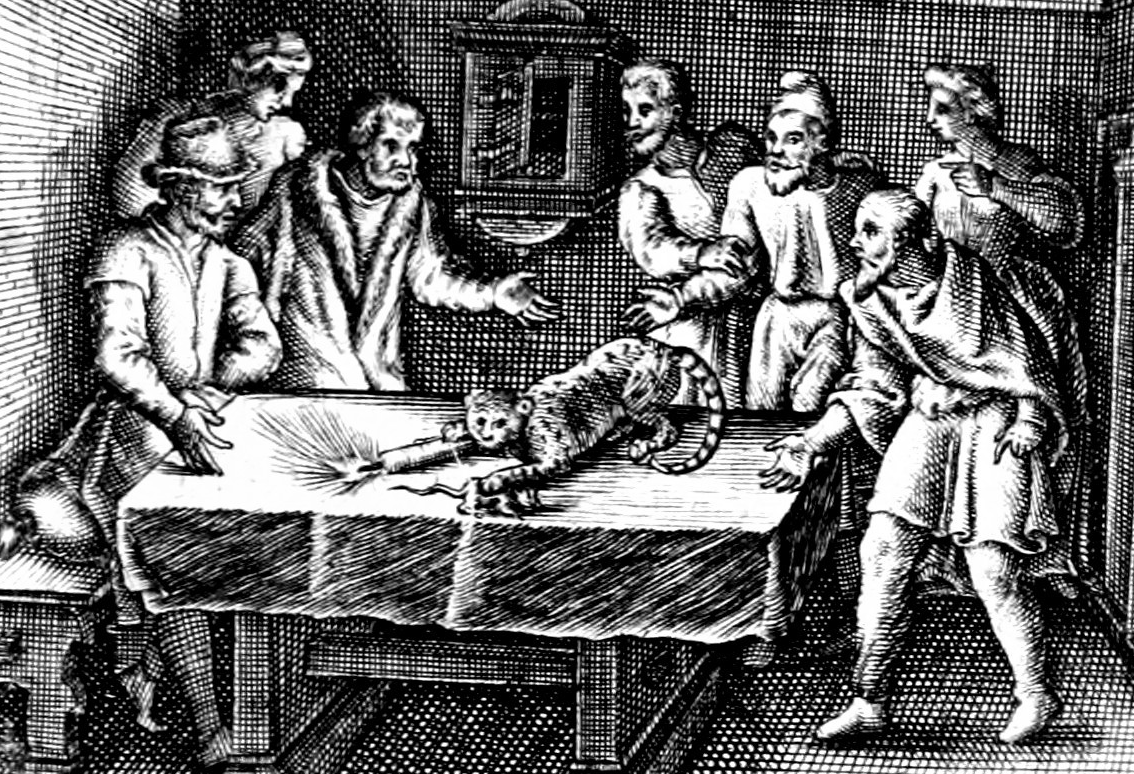
\includegraphics[width=1\textwidth]{images/brev6.png}
 \end{center}

\breakpage